\documentclass{homework}

\title{Homework 3}
\author{Kevin Evans}
\studentid{11571810}
\date{September 20, 2021}
\setclass{Physics}{490}

\usepackage{graphicx}
\usepackage{booktabs}

\usepackage{times}
\usepackage{hyperref}

\begin{document}
	\maketitle
	\begin{enumerate}
		\item From \textit{Physical Review Letters}, \begin{center}
			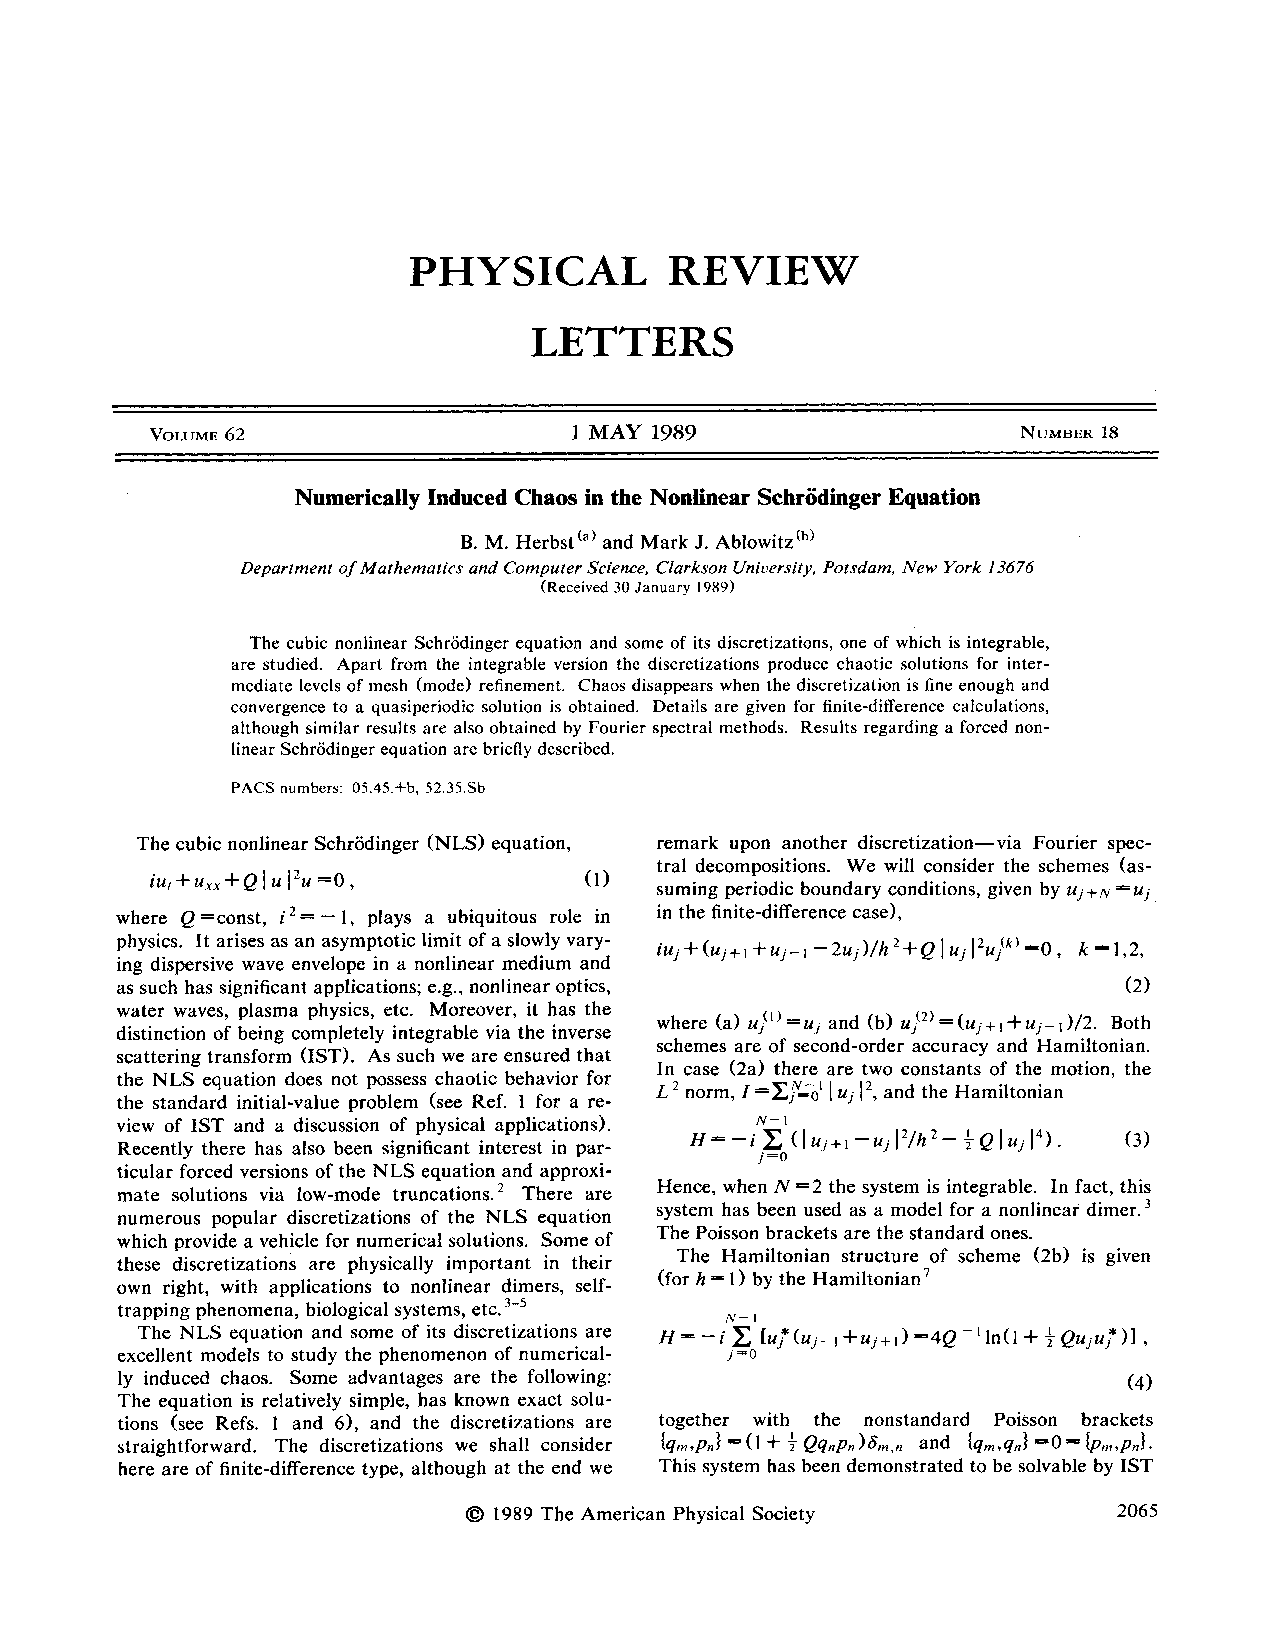
\includegraphics[width=0.9\linewidth]{herbst1989.pdf}
			
			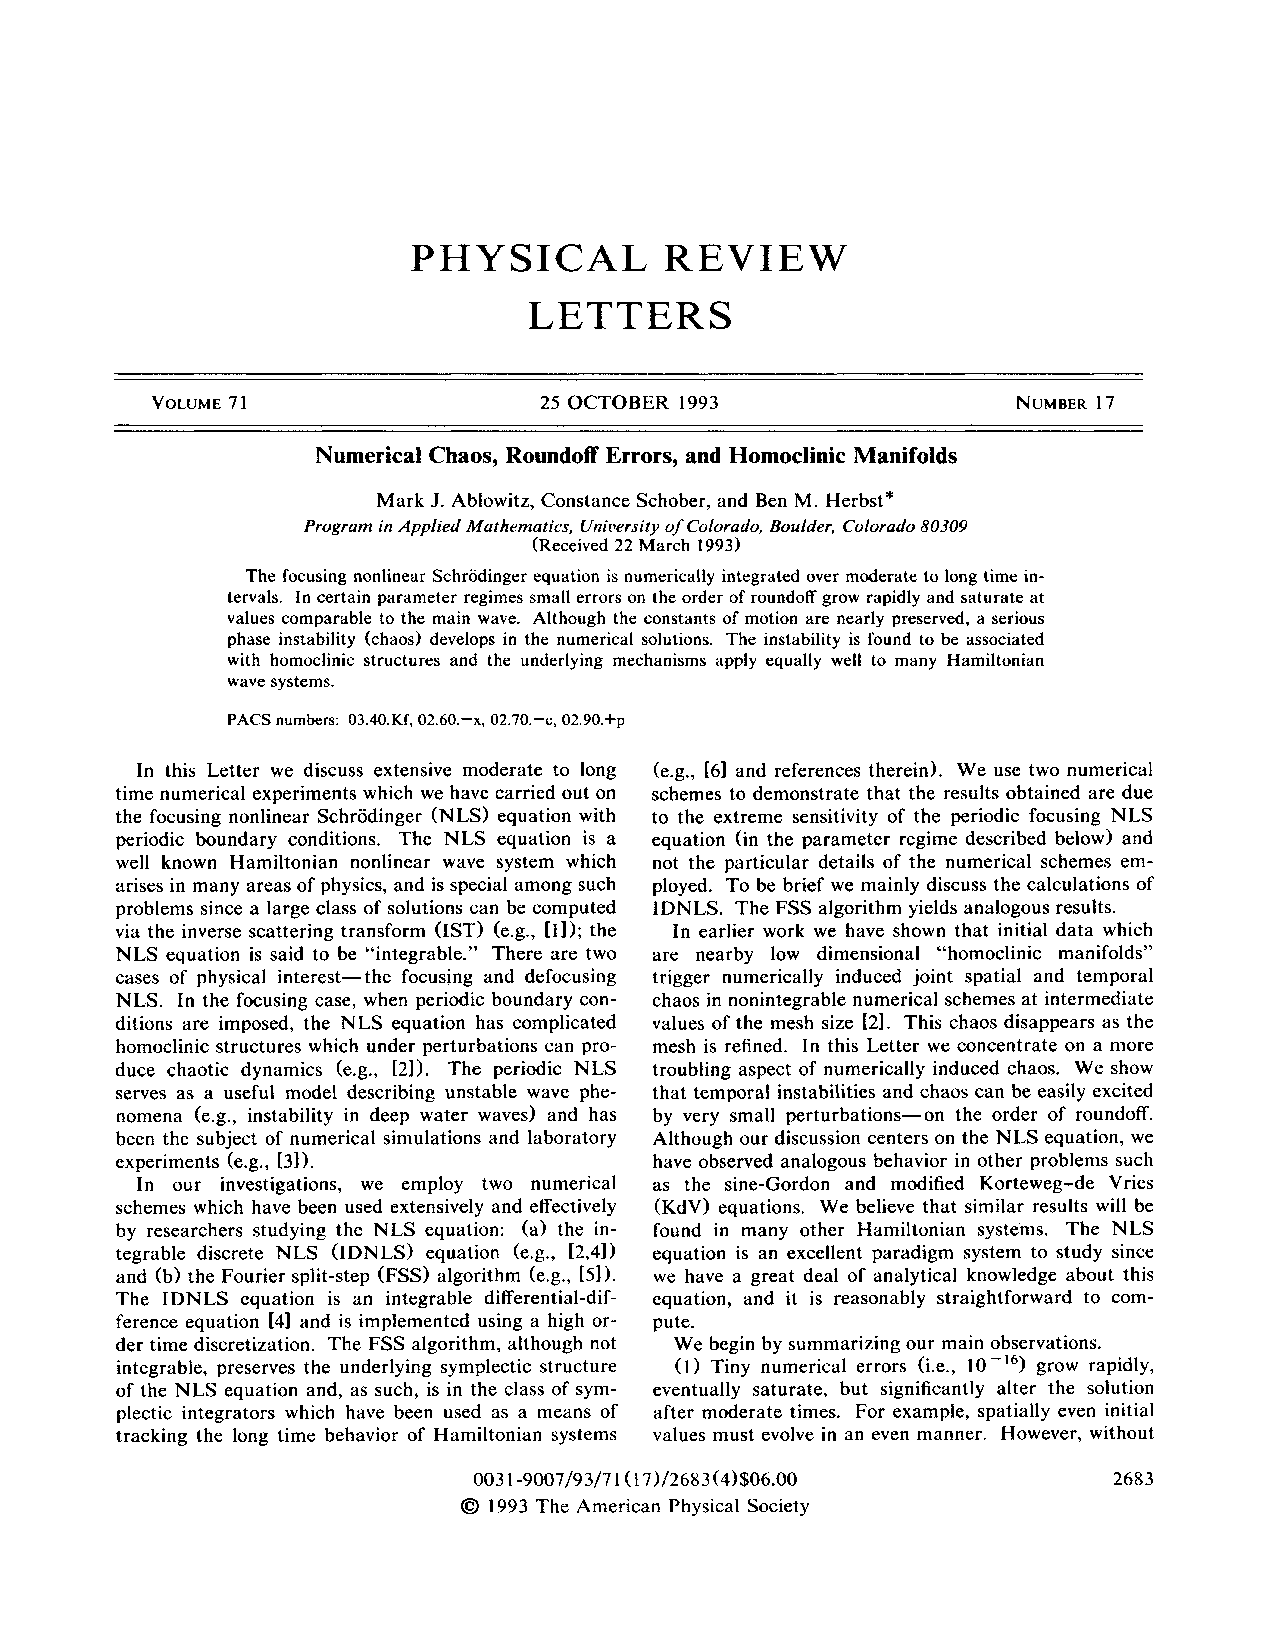
\includegraphics[width=\linewidth]{ablowitz1993.pdf}
		\end{center}
	
		\pagebreak
	
		From \textit{Physical Review A}, \begin{center}		
			\includegraphics[width=\linewidth]{PhysRevA.83.043611.pdf}
			
			\includegraphics[width=\linewidth]{zhao2016.pdf}
		\end{center}
	
	\pagebreak
	
		This isn't from a specialty journal (it's on arXiv), but it's a comprehensive book on BECs and the GPE, \textit{A Primer on Quantum Fluids} by Barenghi and Parker (2016):
		\begin{center}
			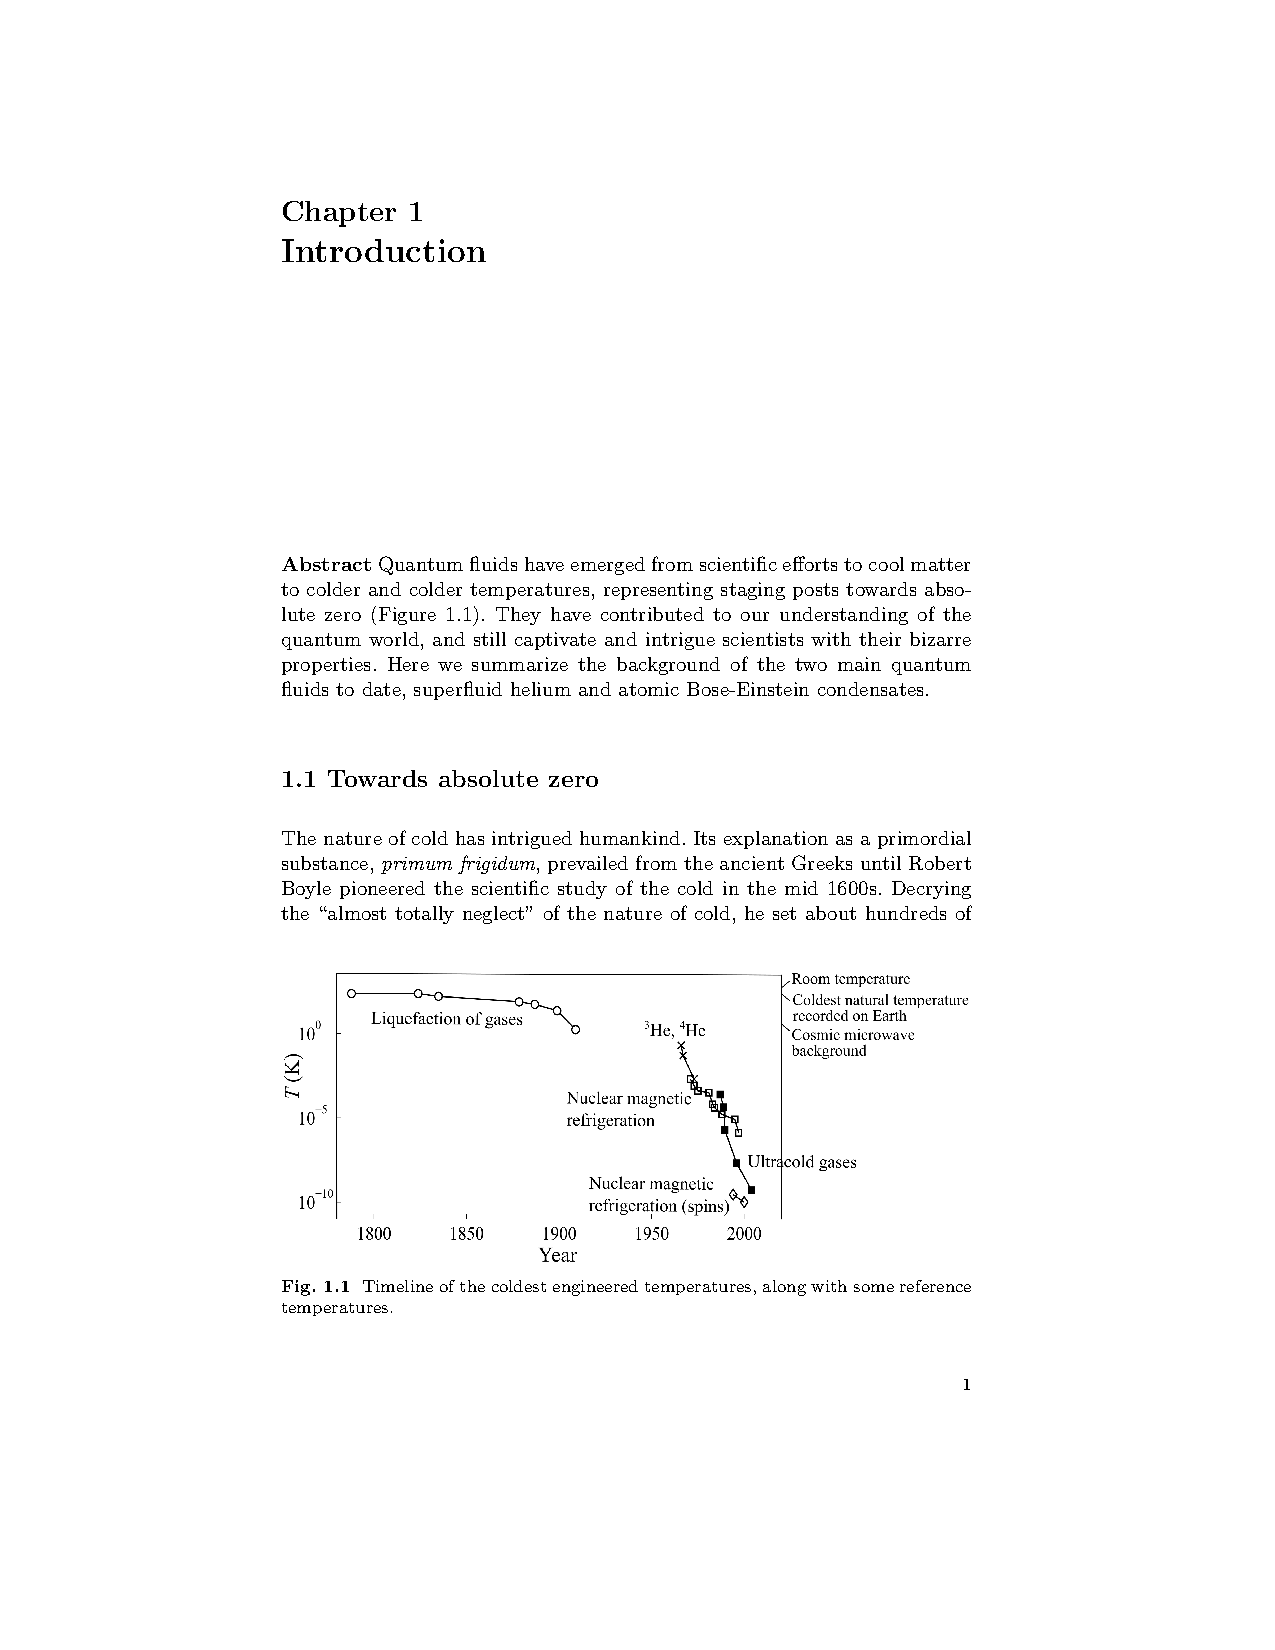
\includegraphics[width=\linewidth,page=1]{1605.09580.pdf}
			\includegraphics[width=\linewidth,page=2]{1605.09580.pdf}		
		\end{center}

\pagebreak

		From \textit{APS},
		\begin{center}
			\includegraphics[width=\linewidth]{mithun2018.pdf}
		\end{center}
		\pagebreak
		
		\item The Gross-Pitaevskii equation (GPE) is a nonlinear Schr\"odinger equation that describes Bose-Einstein condensates (BECs). The equation features a nonlinear addition to the Schrodinger equation approximating the particle interaction as a mean-field Hartree-Fock term. It is interesting that quantum mechanics described by the Schr\"odinger equation is linear and linearity does not bring chaos---however, classical mechanics routinely shows chaos. Here, chaos is calculated by Lyapunov exponents, the exponential divergence in distances in Hilbert space.
		
		
		Here, we characterize chaos within the GPE in one-dimension with Lyapunov exponents. This will be accomplished by simulating the GPE using a finite-differences technique with an adaptive solver. The many-particle wavefunctions will be initialized with turbulence by imparting random phase noise and allowing the function to evolve before perturbing. 
		 We will show that chaos is introduced linearly as a function of the interaction term $g$ for positive coupling-term coefficients. 
		 
		 \item Attached.
	\end{enumerate}
\end{document}